% Este arquivo é uma adaptação do modelo LaTeX disponibilizado pelo UTUG (http://www.inf.ufrgs.br/utug/)
% Autor: Prof. Dr. Adriel M. Ziesemer Jr - IFRS Canoas
% O original encontra-se disponível em: https://sites.google.com/site/profadrielziesemer/home/modelolatexdetccparaoifrs
%
% Dica: Utilize o www.sharelatex.com para editar este documento. Utilize a opcão: Upload Zipped Project

\documentclass[openright]{ifrs} % utilize openright para iniciar capítulos no anverso
\usepackage[T1]{fontenc}        % pacote para conj. de caracteres correto
\usepackage[utf8]{inputenc}     % pacote para acentuaçao
\usepackage{graphicx}           % pacote para importar figuras
\usepackage{times}              % pacote para usar fonte Adobe Times
\usepackage{listings}
\usepackage{multirow}           % pacote para agrupar células em tabelas
\usepackage{scalefnt}           % pacote para redimensionar fontes em tabelas
\usepackage{amsmath}
\usepackage{rotating}           % pacote para rotacionar figuras
\usepackage{url}                % pacote para aceitar URLs (no .bib)
\usepackage{dirtytalk}          % pacote para aspas com comando \say{}
\bibliographystyle{abnt}

% ensine o latex a separar em sílabas as palavras que eventualmente ele não souber
\hyphenation{en-si-na-men-tos a-gra-de-ci-men-to de-se-nha-dos}

\author{Aluno}{Nome do}
%\author{Aluno2}{Nome do}

% edite o definicoes.sty se precisar alterar o nome do curso

\title{Modelo de Trabalho de Conclusão de Curso}

\advisor[Prof.~Dr.]{Orientador}{Nome do}
\coadvisor[Prof.~MSc.]{Co-orientador}{Nome do}

\location{Canoas}{RS}
%\date{julho}{2012} % se nao especificada, é utilizada a data atual

% palavras-chave (começar com letra maiúscula)
\keyword{Sistema}
\keyword{ABNT}
\keyword{IFRS}

% nominata
\newcommand{\nominata}{
        \MakeUppercase{\instituicao}\\
        Reitora: Prof\textsuperscript{a}.~AAAAAA\\
        Diretor do Instituto: Prof.~BBBBBBB\\
        Coordenador do curso: Prof.~CCCCCCC\\
        Bibliotecária-chefe: DDDDDDD
}

% inicio do documento
\begin{document}

% folha de rosto
\maketitle

% dedicatoria (opcional)
\clearpage
\begin{flushright}
\mbox{}\vfill
{\sffamily\itshape
Dedico este trabalho à minha família.}
\end{flushright}

% agradecimentos (opcional)
\chapter*{Agradecimentos}
Cita-los em ordem decrescente de importância.

% resumo
\begin{abstract}
Consiste na apresentação clara e concisa dos pontos relevantes do trabalho, de maneira a permitir ao leitor saber da conveniência ou não da sua leitura na íntegra. Em geral possui 3 seções: a primeira apresenta o que o trabalho trata/tema (Este trabalho apresenta...) e a importância do assunto; a segunda apresenta as novidades/metodologia utilizada no trabalho (Um novo método utilizando [...] foi desenvolvido...); a última descreve o que foi feito para validar o conteúdo (Os resultados obtidos mostraram que...) e principais conclusões.  Cada resumo ocupará no máximo uma folha e terá entre 150 e 500 palavras. Deve ser composto por uma sequência de frases completas em um mesmo parágrafo e não por uma enumeração de tópicos. Dar preferência ao uso da terceira pessoa do singular e do verbo na voz ativa (não utilizar ``eu fiz'' ou ``nós fizemos''; ao invés disso, utilizar ``foi feito''). Após, devem constar palavras-chave relativas aos assuntos do trabalho, separadas entre si por ponto.  
 \end{abstract}

% resumo na outra lingua (opcional)
\begin{englishabstract}
{Title of the Work in English}
{System. ABNT. IFRS} % Palavras Chaves: iniciar com letras maiúsculas e separar por '.'
This work has the purpose of [...]. The text in the abstract should not contain more than 500 words. Use the third person in the plural (We developed...).
\end{englishabstract}

% lista de abreviaturas e siglas
\begin{listofabbrv}{SPMD}
        \item[ILP] Programação Linear com Inteiros (\textit{Integer Linear Programming})
        \item[TADS] Curso Superior de Tecnologia em Análise e Desenvolvimento de Sistemas
\end{listofabbrv}

% lista de figuras
\listoffigures

% lista de tabelas
\listoftables

% lista de símbolos (opcional)
%\begin{listofsymbols}{$\alpha\beta\pi\omega$}
%       \item[$\sum{\frac{a}{b}}$] Somatório do produtório
%       \item[$\alpha\beta\pi\omega$] Fator de inconstância do resultado
%\end{listofsymbols}

% sumário
\tableofcontents

\chapter{Introdução}
Faça a introdução de forma a contextualizar a área na qual se enquadra o trabalho proposto. Fale sobre o problema existente na qual se tentará encontrar uma solução. Destaque a importância e relevância do trabalho.

Tome muito cuidado ao definir o título do trabalho. Ele deve refletir o principal assunto tratado. É melhor utilizar um título modesto (mais específico), mas sobre algo que foi devidamente trabalhado no texto, do que abraçar o mundo e deixar o trabalho incompleto. As vezes pode ser necessário redefini-lo quando o trabalho estiver terminado.

Como regra geral para todo o texto, evite frases muito longas (com mais de 3 linhas de extensão), isto dificulta a compreensão. Interrompa a frase com um ponto final assim que der e continue na mesma linha.

Evite utilizar ``a nível de'' ou ``em nível de''. Ao invés disto, utilize: ``com/em relação a'', ``no que concerne'', ``quanto a'', dentre outras. Também dê uma boa revisada nas regras da crase antes de começar a escrever.

Não faça afirmações fortes (ex.: nunca, sempre, impossível, ótimo,...) sem junto citar a fonte ou realizar a devida prova formal. Citar a fonte serve justamente para tirar esta responsabilidade de quem escreve um texto técnico. Também não reproduza textos de terceiros sem citar a fonte (plágio).
\section{Motivação}
Discutir as abordagens existentes e o porquê delas não serem satisfatórias.
\section{Objetivos}
Deve apresentar a nova abordagem e no que ela é superior às existentes
Alguns autores subdividem os objetivos em gerais e específicos.
\subsection{Objetivos Gerais}
Principal contribuição.
\subsection{Objetivos Específicos}
Devem ser apresentados em forma de lista, iniciando cada um com o verbo no infinitivo: esclarecer tal coisa; definir tal assunto; procurar aquilo; permitir aquilo outro, demonstrar alguma coisa etc.
\section{Organização do Texto}
O Capítulo \ref{cap:revbib} apresenta uma revisão bibliográfica sobre o tema e um estudo sobre os principais trabalhos existentes...

\chapter{Revisão Bibliográfica} \label{cap:revbib}
Apresentar o que já foi desenvolvido por outros pesquisadores (trabalhos relacionados). Priorize citações nesta ordem: periódicos, livros, teses, anais e por último qualquer outra fonte. Internacional é melhor que nacional; qualis A é melhor que B; recente é melhor do que antigo.
\section{Estudo dos Trabalhos Existentes}
Sintetizar os trabalhos citados, não precisa colocar o texto ``ao pé da letra''. Agrupe trabalhos similares e faça um resumo com suas palavras.
\section{Estado da Arte}
Apresentar o que há de mais novo (técnicas, métodos, algoritmos, ferramentas,...) sobre o assunto (publicado preferencialmente nos últimos 5 anos). Descreva os detalhes, coloque: fluxogramas, algoritmos, figuras, pontos fortes/fracos...
\section{Conclusões}
Reunir as ideias principais abordadas no capítulo.

\chapter{Pesquisa de Mercado}
Opcional, dependendo do tipo de trabalho. Serve para embasar a necessidade de algo ou coletar informações sobre o assunto. 

\chapter{Análise de Viabilidade} 
Opcional, dependendo do tipo de trabalho. Serve para provar que a abordagem proposta é viável de ser implementada.
\section{Viabilidade Técnica}
\section{Viabilidade Econômica}

\chapter{Desenvolvimento do Trabalho Proposto}
A minha contribuição.
\section{Introdução}
\section{Planejamento}
\subsection{Cronograma}
As atividades serão desenvolvidas conforme o cronograma mostrado na Tabela \ref{cronograma}.

\begin{table}
\caption{Cronograma de atividades}
\begin{center}
\begin{tabular}{l|c|c|c|c|c|c|c|c|c}
\hline \multirow{2}{*}{Tarefa}& 2012& \multicolumn{8}{c}{2013}\\
          	             & Dez & Jan & Fev & Mar & Abr & Mai & Jun & Jul & Ago \\
\hline
\hline Estudo DFM        &  X  &  X  &  X  &     &     &     &     &     &     \\
\hline Correções DRC     &     &  X  &  X  &  X  &  X  &     &     &     &     \\
\hline Finalização Astran&     &     &     &     &  X  &  X  &  X  &     &     \\
\hline Resultados        &     &     &     &     &     &     &  X  &  X  &     \\
\hline Artigos           &     &     &     &  X  &     &     &     &  X  &     \\
\hline Texto da Tese     &     &     &     &     &     &     &  X  &  X  &  X  \\
\hline Defesa	         &     &     &     &     &     &     &     &     &  X  \\
\hline 
\end{tabular}
\end{center}
\label{cronograma}
\end{table}

\subsection{Alocação dos Recursos}
\section{Execução}
\subsection{Coleta de Dados}
\subsubsection{Entrevista}
\subsubsection{Questionário}
\subsubsection{Requisitos}
\subsection{Documentação}
\subsubsection{Estrutura Geral}
\subsubsection{Casos de Uso}
O caso de uso Cadastrar Ônibus é mostrado da Tabela \ref{tabelaCadastrarOnibus}.

\begin{table}
\caption{Caso de uso - Cadastrar ônibus.}
\begin{tabular}{p{7cm}|p{7cm}}
\hline
\multicolumn{2}{c}{\bf Ação - Cadastrar ônibus} \\
\hline
\multicolumn{2}{l}{Atores:  Administrador} \\
\hline
\multicolumn{2}{l}{Pré-condição:  Autenticação do ator Administrador} \\
\hline
\multicolumn{2}{l}{Pós-condição:  Ônibus cadastrado na base de dados} \\
\hline
\multicolumn{2}{c}{\bf Fluxo de Eventos} \\
\hline
Ator & Sistema \\
\hline
1. Acessa o menu de ônibus & \\
\hline
 &  2. Exibe uma lista de ônibus cadastrados juntamente com uma opção
"adicionar ônibus" \\
\hline
3. Clica na opção "adicionar ônibus" &\\
\hline
& 4. Exibe um campo contendo id, um campo para informar número, um campo para 
seleção da acessibilidade a cadeirantes, um campo para informar a disponibilidade do 
ônibus e outro para que seja informado à qual empresa pertence.\\
\hline
5. Informa o número, a empresa à qual pertence e seleciona se é 
acessível para cadeirantes. & \\
\hline
& 6. Exibe uma mensagem de sucesso. \\
\hline
\end{tabular}
\label{tabelaCadastrarOnibus}
\end{table}

\subsubsection{Diagrama de Classes}
\subsubsection{Diagrama de Entidades e Relacionamentos}
\subsubsection{Dicionário de Dados}
\subsubsection{Especificação Detalhada dos Processos}
\subsubsection{Testes e Depurações}
\subsubsection{Considerações/Características Técnicas do Projeto}
\subsubsection{Projeto de Interface}
\subsection{Desenvolvimento}
\subsubsection{Justificativa da Escolha dos Métodos/Ferramentas}
\subsubsection{Como Foram Implementados/Adaptados os Métodos para a Solução do Problema}
\subsubsection{Divisão de Tarefas}
\subsubsection{Cronograma Executado de Atividades}
\subsubsection{Resumo das Atas de Reunião (com data)}
\subsubsection{Recursos Utilizados para Projeto/Desenvolvimento/Implantação/Treinamento/Manutenção:
Tempo, Financeiros, Materiais e Pessoais}

\chapter{Resultados}
Há trabalhos que apresentam várias metodologias e, para cada uma delas, colocam a revisão bibliográfica, desenvolvimento e resultados dentro do mesmo capítulo. Não há uma regra fixa para o corpo do trabalho, desde que tenham estes dados. 
\section{Conjuntos de Testes Utilizados}
\section{Comparações com Métodos/Ferramentas Existentes}
\section{Capturas de Tela}

\chapter{Conclusão}
Considerações finais sobre o assunto, se os objetivos foram alcançados, o que se descobriu, quais outras questões surgiram a partir dos resultados e se as hipóteses se confirmaram ou não.
\section{Contribuições}
\section{Trabalhos Futuros}
\section{Considerações Finais}

% carrega o arquivo com as bibliografias e põe o capítulo com as referências neste lugar
\bibliography{bibliografia}

% a partir daqui, todo capítulo novo é apêndice
\appendix

\chapter{Anexos e Apêndices}
Destinam-se à inclusão de informações complementares ao trabalho, mas que não são essenciais à sua compreensão. Os Apêndices devem apresentar material desenvolvido pelo próprio autor, formatado de acordo com as normas. Já os Anexos destinam-se à inclusão de material como cópias de artigos, manuais, etc., que não necessariamente precisam estar em conformidade com o modelo, e que não foram desenvolvidos pelo autor do trabalho.

%importa dicasLatexABNT.tex para o Apêndice 
\chapter{Dicas de Latex e Normas ABNT}
Esta capítulo apresenta as coisas básicas que precisamos saber para fazer um TCC com Latex utilizando este modelo.

\section{O Básico do Latex}
Novo parágrafo pode ser feito por meio do comando par. \par
Outra forma é deixando uma linha em branco entre dois parágrafos.

Tudo o que está a direita de um \% é um comentário.
% Isto é um comentário
Para inserirmos o símbolo de porcento de forma proposital, precisamos colocar a barra invertida antes: 90\%.

Os caracteres \& \$ \# \% \_ \{ \} \^{} \~{} $\backslash$ são todos especiais e precisam ser escritos como comandos (com uma barra antes).
% tem um web app para ajudar a encontrar outros símbolos neste endereço: http://detexify.kirelabs.org/classify.html

Aspas são digitadas com duas crases no início e duas aspas simples no final: ``Texto entre aspas''; ou com o comando say: \say{Texto entre aspas}.

Estilos de fontes: \emph{ênfase} (sempre destaca o texto, mesmo que este já esteja em negrito/itálico), \textbf{negrito}, \textit{itálico}, \textrm{romano}, \textsf{sans serif}, \texttt{máquina de escrever}, \textsc{caixa alta}.

Capítulos, seções e subseções são inseridas com:
\begin{verbatim}
\chapter{Um Capítulo} -> 1 Um Capítulo
\section{Uma Seção} -> 1.1 Uma Seção
\subsection{Uma Subseção} -> 1.1.1 Uma Subseção
\subsubsection{Uma Subsubseção} -> 1.1.1.1 Uma Subsubseção
\chapter*{Um Capítulo} -> Um Capítulo sem numeração
\end{verbatim}
Não se deve utilizar mais do que 4 níveis.

Ambientes são utilizados para definir uma região do texto que haverá tratamento especial:

\begin{verbatim}
O ambiente verbatim significa "ao pé da letra". 
Ex.: & $ # % _ { } ^ ~ $
\end{verbatim}

\begin{center}
O ambiente center escreve centralizado.
\end{center}

\begin{quote}
O ambiente quote é útil para fazer citações.
\end{quote}

Esta é a forma como se descreve itens:
\begin{description}
\item[Item 1] Isto significa uma coisa.
\item[Item 2] Este significa outra coisa.
\end{description}

Esta é a forma como se cita itens:
\begin{itemize}
\item Item 1;
\item Item 2.
\end{itemize}

E esta é a forma como se enumera itens:
\begin{enumerate}
	\item Qual a alternativa correta?
		\begin{enumerate}
			\item esta.
			\item ou esta.
		\end{enumerate}
\end{enumerate}

Fórmulas matemáticas são colocadas dentro de um ambiente matemático. Tudo neste ambiente é considerado elemento numérico e possui uma formatação diferente. Os comandos aceitos também podem mudar.

Equações matemáticas em destaque são inseridas da seguinte maneira:

% tem um web app para ajudar a fazer equações neste endereço: http://mathurl.com/
% ou aqui: http://webdemo.visionobjects.com/#/demo/equation
$$
x=\frac{-b\pm\sqrt{b^2-4ac}}{2a}.
$$

ou 

\begin{equation}
\begin{array}{rcl}
x_2 - x_1 &\geq& b_1 r_1\\
x_2 - x_1 &\geq& b_2 r_2\\
x_2 - x_1 &\geq& b_n r_m\\
b_1 + b_2 + ... + b_n &=& 1
\end{array}
\end{equation}

enquanto equações inline são feitas desta forma: $r_i (1\leq i \leq m)$.

\section{Convenções}
Escreva o título e os capítulos, seções, subseções, etc. sempre com a primeira letra de cada palavra importante em Maiúsculo e o restante em minúsculo. O Latex se encarregará de deixar tudo MAIÚSCULO onde for necessário.

Nenhuma seção deve ficar sem texto.

Utilize siglas para não ter de repetir muitas vezes o mesmo texto. Neste caso, na primeira ocorrência coloque o significado antes e a sigla entre parênteses (aproveitando também para adiciona-la à lista de siglas). Nas demais ocorrências, apenas coloque a sigla. 
Ex.: ...com a execução do algoritmo de \textit{Threshold Accepting} (TA) sobre um circuito. A versão do algoritmo de TA utilizada...

Palavras em \textit{English} ou outra língua estrangeira devem estar em itálico. Utilize \textbf{negrito} quando for necessário destacar alguma coisa.

\section{Figuras e Tabelas}

Todas as figuras e tabelas devem estar referenciadas no texto e com a descrição acima delas. Não são permitidos outros nomes tais como: quadro, imagem, etc. Comece a descrição com letra maiúscula e faça o restante em minúscula (exceto siglas), terminando com um ponto final.

Se buscada em alguma obra publicada, a citação deve sempre aparecer. Pode ser colocada entre parênteses, como no exemplo da Figura \ref{fig:dsp2}, ou preferencialmente abaixo após a palavra "Fonte: ", como no exemplo da Tabela \ref{tab:comp1} e da Figura \ref{fig:dsp}. Observando que na LISTA DE FIGURAS/TABELAS a fonte/citação não deve aparecer.

É possível colocar as figuras de lado e também redimensiona-las através dos parâmetros do Latex, como nos exemplos das Figuras \ref{fig:dsp} e \ref{fig:dsp2}. Dê preferência por imagens vetoriais ou em PDF, para não perder qualidade. Procure deixar os textos das figuras com o mesmo tamanho das letras no restante do documento.

\begin{figure} % [h] -> utilize este parâmetro para forçar nesta posição
    \center{
    \caption{Segundo a ABNT, a descrição deve ficar acima da figura.}
    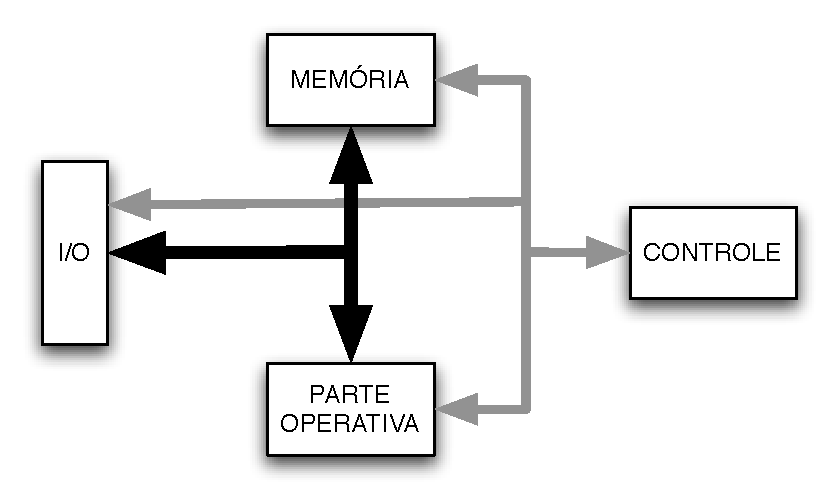
\includegraphics[width=20em]{figuras/dsp}\\
    Fonte: Elaborado pelo autor.}
    \label{fig:dsp}
\end{figure}

\begin{sidewaysfigure}
    % entre colchetes a descrição que vai para a lista de figuras, sem citação (parâmetro opcional mas que é necessário devido a norma da ABNT)
    \caption[Descrição com citação]{Descrição com citação \cite{artigo}.}
    \centerline{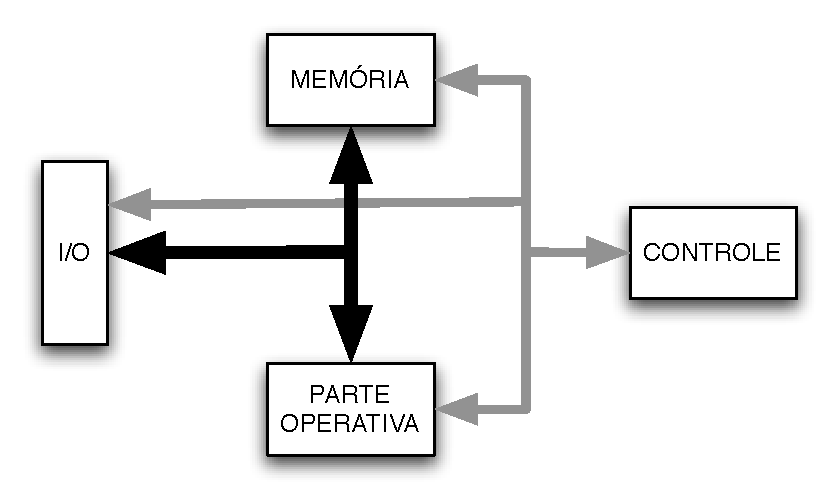
\includegraphics[width=40em]{figuras/dsp}}
    \label{fig:dsp2}
\end{sidewaysfigure}

As tabelas devem ser ``abertas'' dos lados (sem as linhas laterais), como no exemplo da Tabela \ref{tab:comp1}, isto torna a imagem mais limpa e clara.

% tem um web app para ajudar a fazer tabelas no Latex neste endereço: http://truben.no/latex/table/
\begin{table}
    \centering
    \scalefont{0.93} %necessário eventualmente para reduzir o tamanho da tabela
    \caption{Comparação entre X e Y.}
    \begin{tabular}{c|c|c|c|c|c} \hline
        \multirow{2}{*}{\textbf{Célula}} & \multirow{2}{*}{\# \bf{Trans.}} & \multicolumn{3}{|c|}{\bf{Largura} ($\mu m$)} & \bf{Tempo Exec. (s)}\\ \cline{3-6} 
         &  & Std. Cell & ASTRAN & \% & ASTRAN \\ \hline \hline
        AND2X4& 6 & 1 & 1,2 & 20 & 10 \\ \hline
        FAD1X4& 28 & 3,6 & 4 & 12 & 750\\ \hline
        FAD1X9& 28 & 4,2 & 4,2 & 0 & 1800\\ \hline
        HAD1X9& 14 & 2,4 & 2,4 & 0 & 30\\ \hline
        HAD1X18& 18 & 2,8 & 2,8 & 0 & 205\\ \hline
        INVX0 & 2 & 0,6 & 0,6 & 0 & 1\\ \hline
        TOTAL& - & 28 & 29 & 3,6 &-\\ \hline
    \end{tabular}
    {\\ Fonte: \cite{artigo}}
    \label{tab:comp1}
\end{table}

\section{Citações}
Há duas formas de se fazer uma citação: a citação indireta ou livre e a citação direta ou textual. Todas as citações devem trazer a identificação de sua autoria.

No Latex, inserimos citações utilizando o formato bibtex. Para tanto, precisamos cadastrar os dados da citação no arquivo .bib e em seguida citarmos no .tex com o comando cite. Colocar preferencialmente em ordem cronológica, com o mais recente por último \cite{livro, artigo, tese, capitulo, paper, site, apresentacao}.

\subsection{Citação Indireta}
Aquela citação na qual expressamos o pensamento de outra pessoa com nossas próprias palavras. Por esta razão seu uso é mais recomendado, pois demostra interpretação do autor sobre a obra citada. Ex.:

Segundo o trabalho de Silva e Santos \citeyearpar{artigo}, o céu é azul porque...

O céu é azul porque... \cite{artigo}.

\subsection{Citação Direta}
São aquelas em que se transcreve exatamente as palavras do autor citado. As citações diretas ou textuais podem ser breves ou longas. São consideradas breves aquelas cuja extensão não ultrapassa três linhas e devem vir entre aspas. As citações com mais de três linhas são chamadas de longas (sem aspas) e devem receber um destaque especial com recuo.  Ex.:

Segundo Silva, ``Quando a luz passa através de um prisma, seu espectro é dividido em sete cores monocromáticas'' \citeyearpar{artigo}.

\begin{quote}
Quando a luz passa através de um prisma, seu espectro é dividido em sete cores monocromáticas, eis que surge um arco-íris de cores. A atmosfera faz o mesmo papel do prisma, atuando onde os raios solares colidem com as moléculas de ar, água e poeira e são responsáveis pela dispersão do comprimento de onda azul da luz. \cite{artigo}
\end{quote}

Havendo supressão de trechos dentro do texto citado, faz-se a indicação com reticências entre colchetes [...]. De forma similar, para interpelação, acréscimo ou comentário durante a citação, deve-se fazê-lo também entre colchetes. No início ou no fim da citação, as reticências são usadas apenas quando o trecho citado não é uma sentença completa.Ex.:

``Também chamado de corpo do trabalho, [o desenvolvimento] tem por finalidade expor [...] a explicitação do assunto a ser abordado...'' \cite{artigo}.

\section{Notas de Rodapé}
As notas de rodapé\footnote{Nota sobre a palavra rodapé} são usadas nos documentos impressos para explicar ou fazer comentários detalhados.


\end{document}
